%!TEX root = ../../thesis.tex



\subsection{Stellar and planetary formation}

Brown dwarfs


- Small densities - mercury like  density~\citet{dittmann_temperate_2017, santerne_earthsized_2018, ment_second_2018} rocky super-earths\todo{move elsewhere}\\


\subsection{Exoplanet distribution} 4 different groups

\fref{}


\begin{figure}
    \centering
    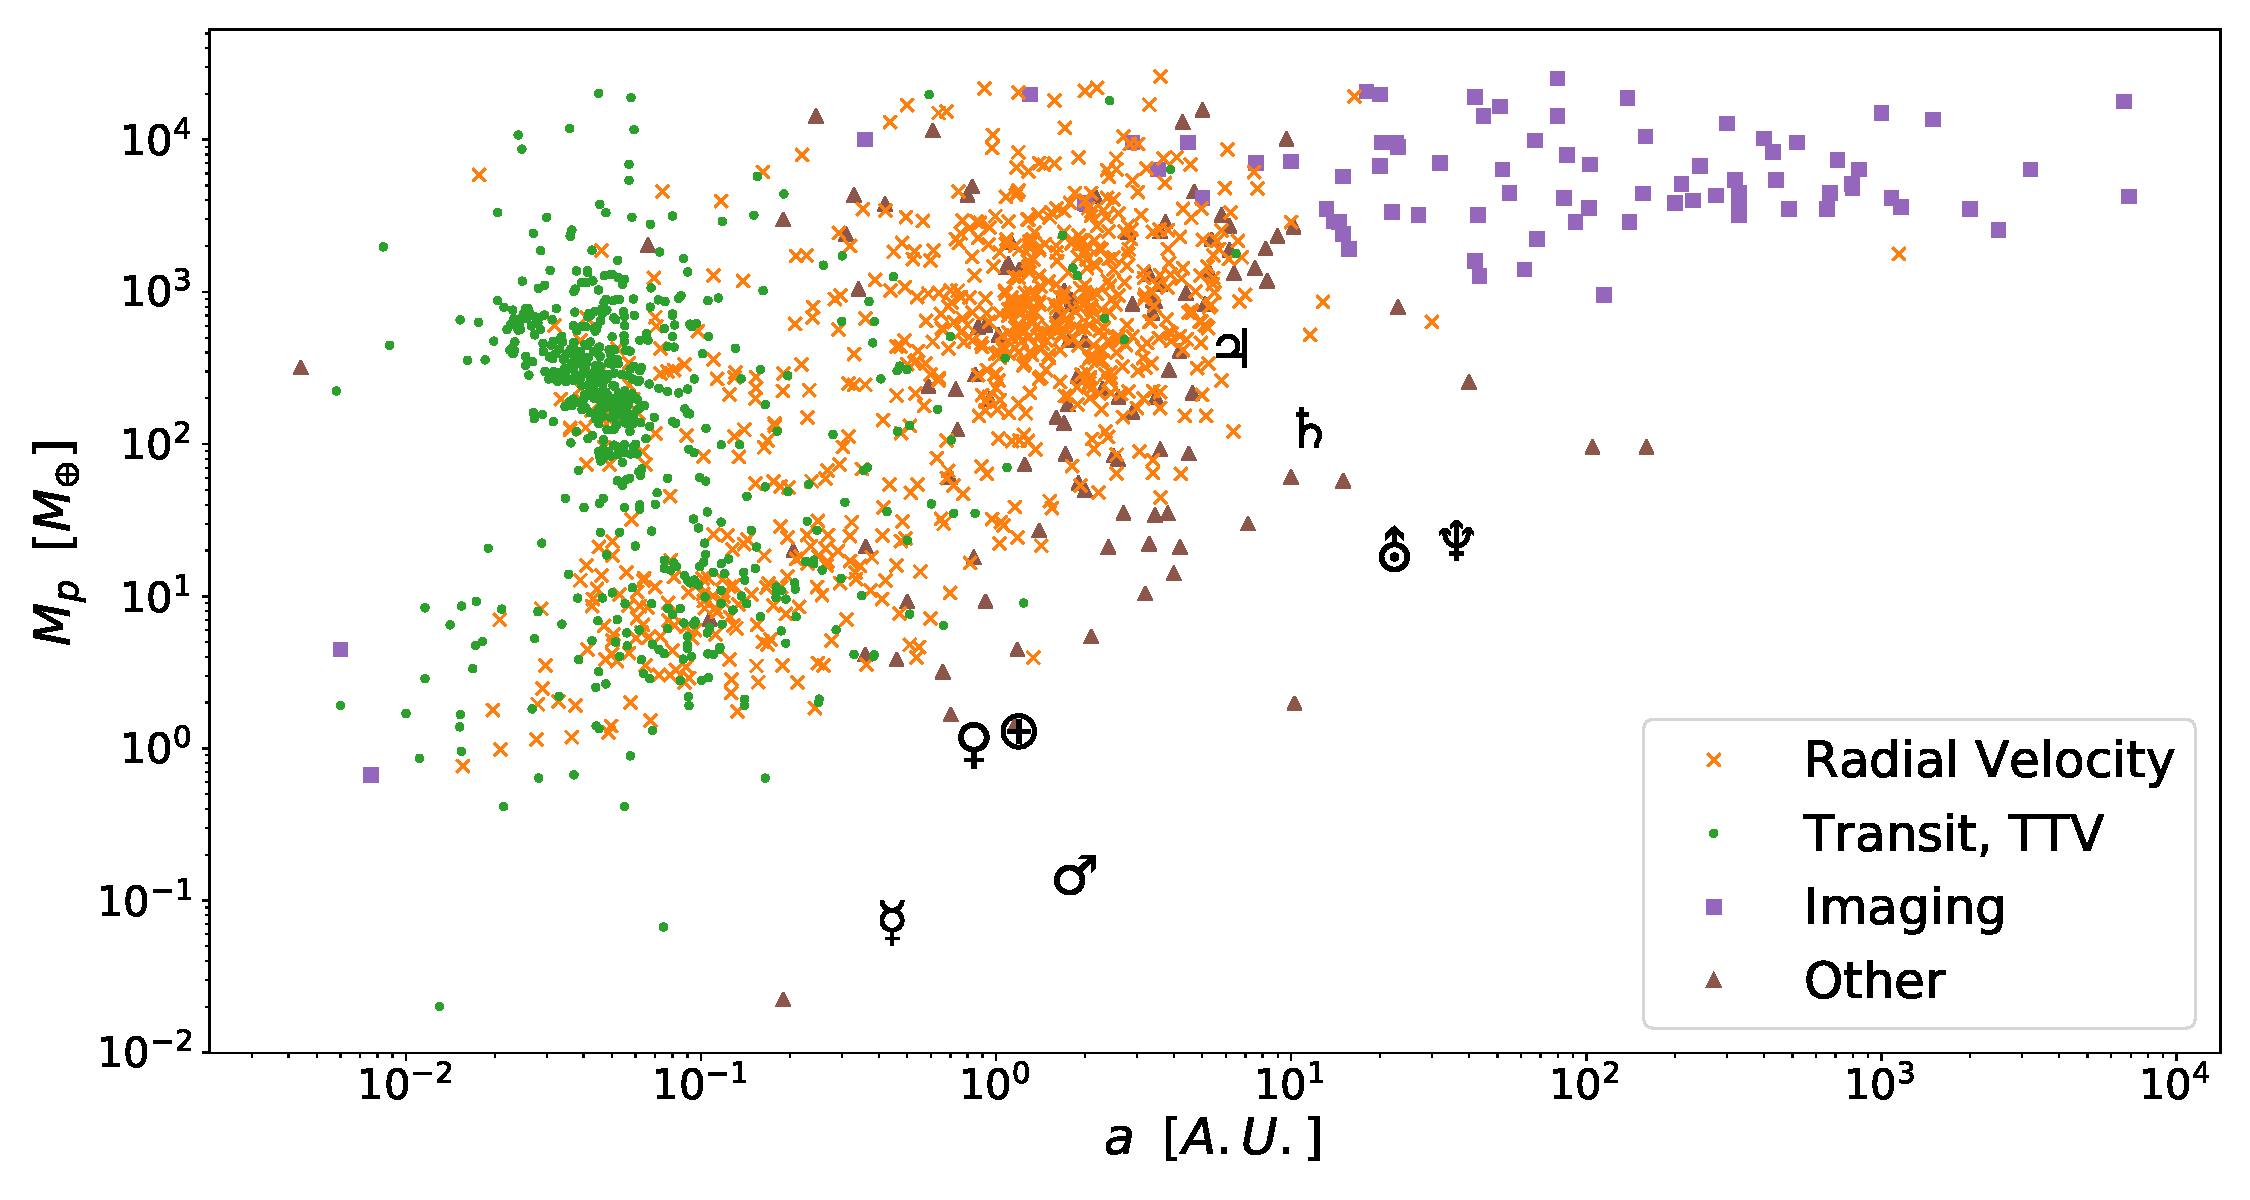
\includegraphics[width=0.7\linewidth]{./figures/introduction/exoplanetEU_a_mass.pdf}
    \caption{Distance mass diagram.
        The symbols indicate the location of the solar system planets, $\mercury$-Mercury, $\venus$-Venus, $\earth$-Earth, $\mars$-Mars, $\jupiter$-Jupiter, $\saturn$-Saturn, $\uranus$-Uranus, $\neptune$-Neptune. Data from \href{http://ww.exoplanet.eu}{exoplanet.eu} October 2018}
    \label{fig:pltoverlayadd}
\end{figure}


Explore what these method have found with exoplanet populations.

The discovery of the hot-Jupiter class (large mass planets on close in orbits) challenged the accepted planet formation theories at the time~\citep[.e.g][]{pollack_formation_1996} in which our Solar System was thought to be typical with small rocky planets close to the Sun and large giant planets further away.


\begin{figure}[t]
    \centering
    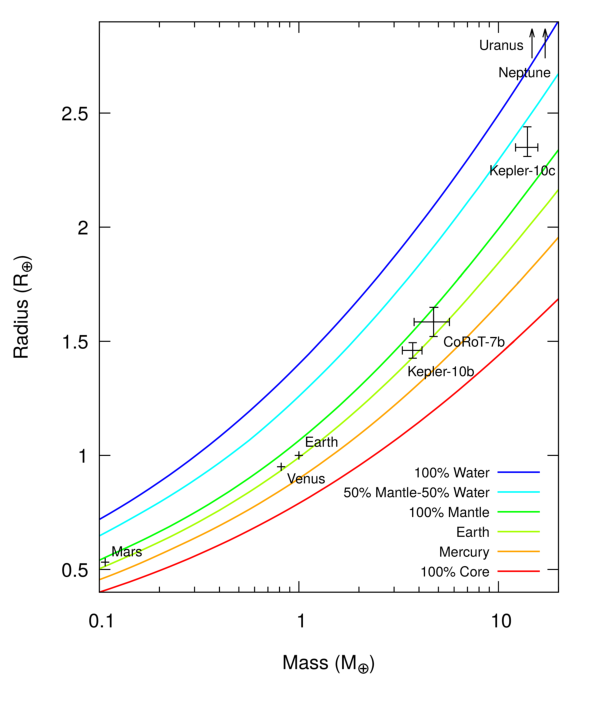
\includegraphics[width=0.4\linewidth]{./figures/introduction/Mass_radius_relation-compostion_Brugger_2017.pdf}\\
    \caption{Mass-Radius relationship for (super) Earth-like planets with composition contours~\citet{brugger_constraints_2017}}
    \label{fig:mass_radius_relation_composition}
\end{figure}

MR relation ship image arXiv:1506.05097~\citet{chen_probabilistic_2016}

\begin{figure}[t]
    \centering
    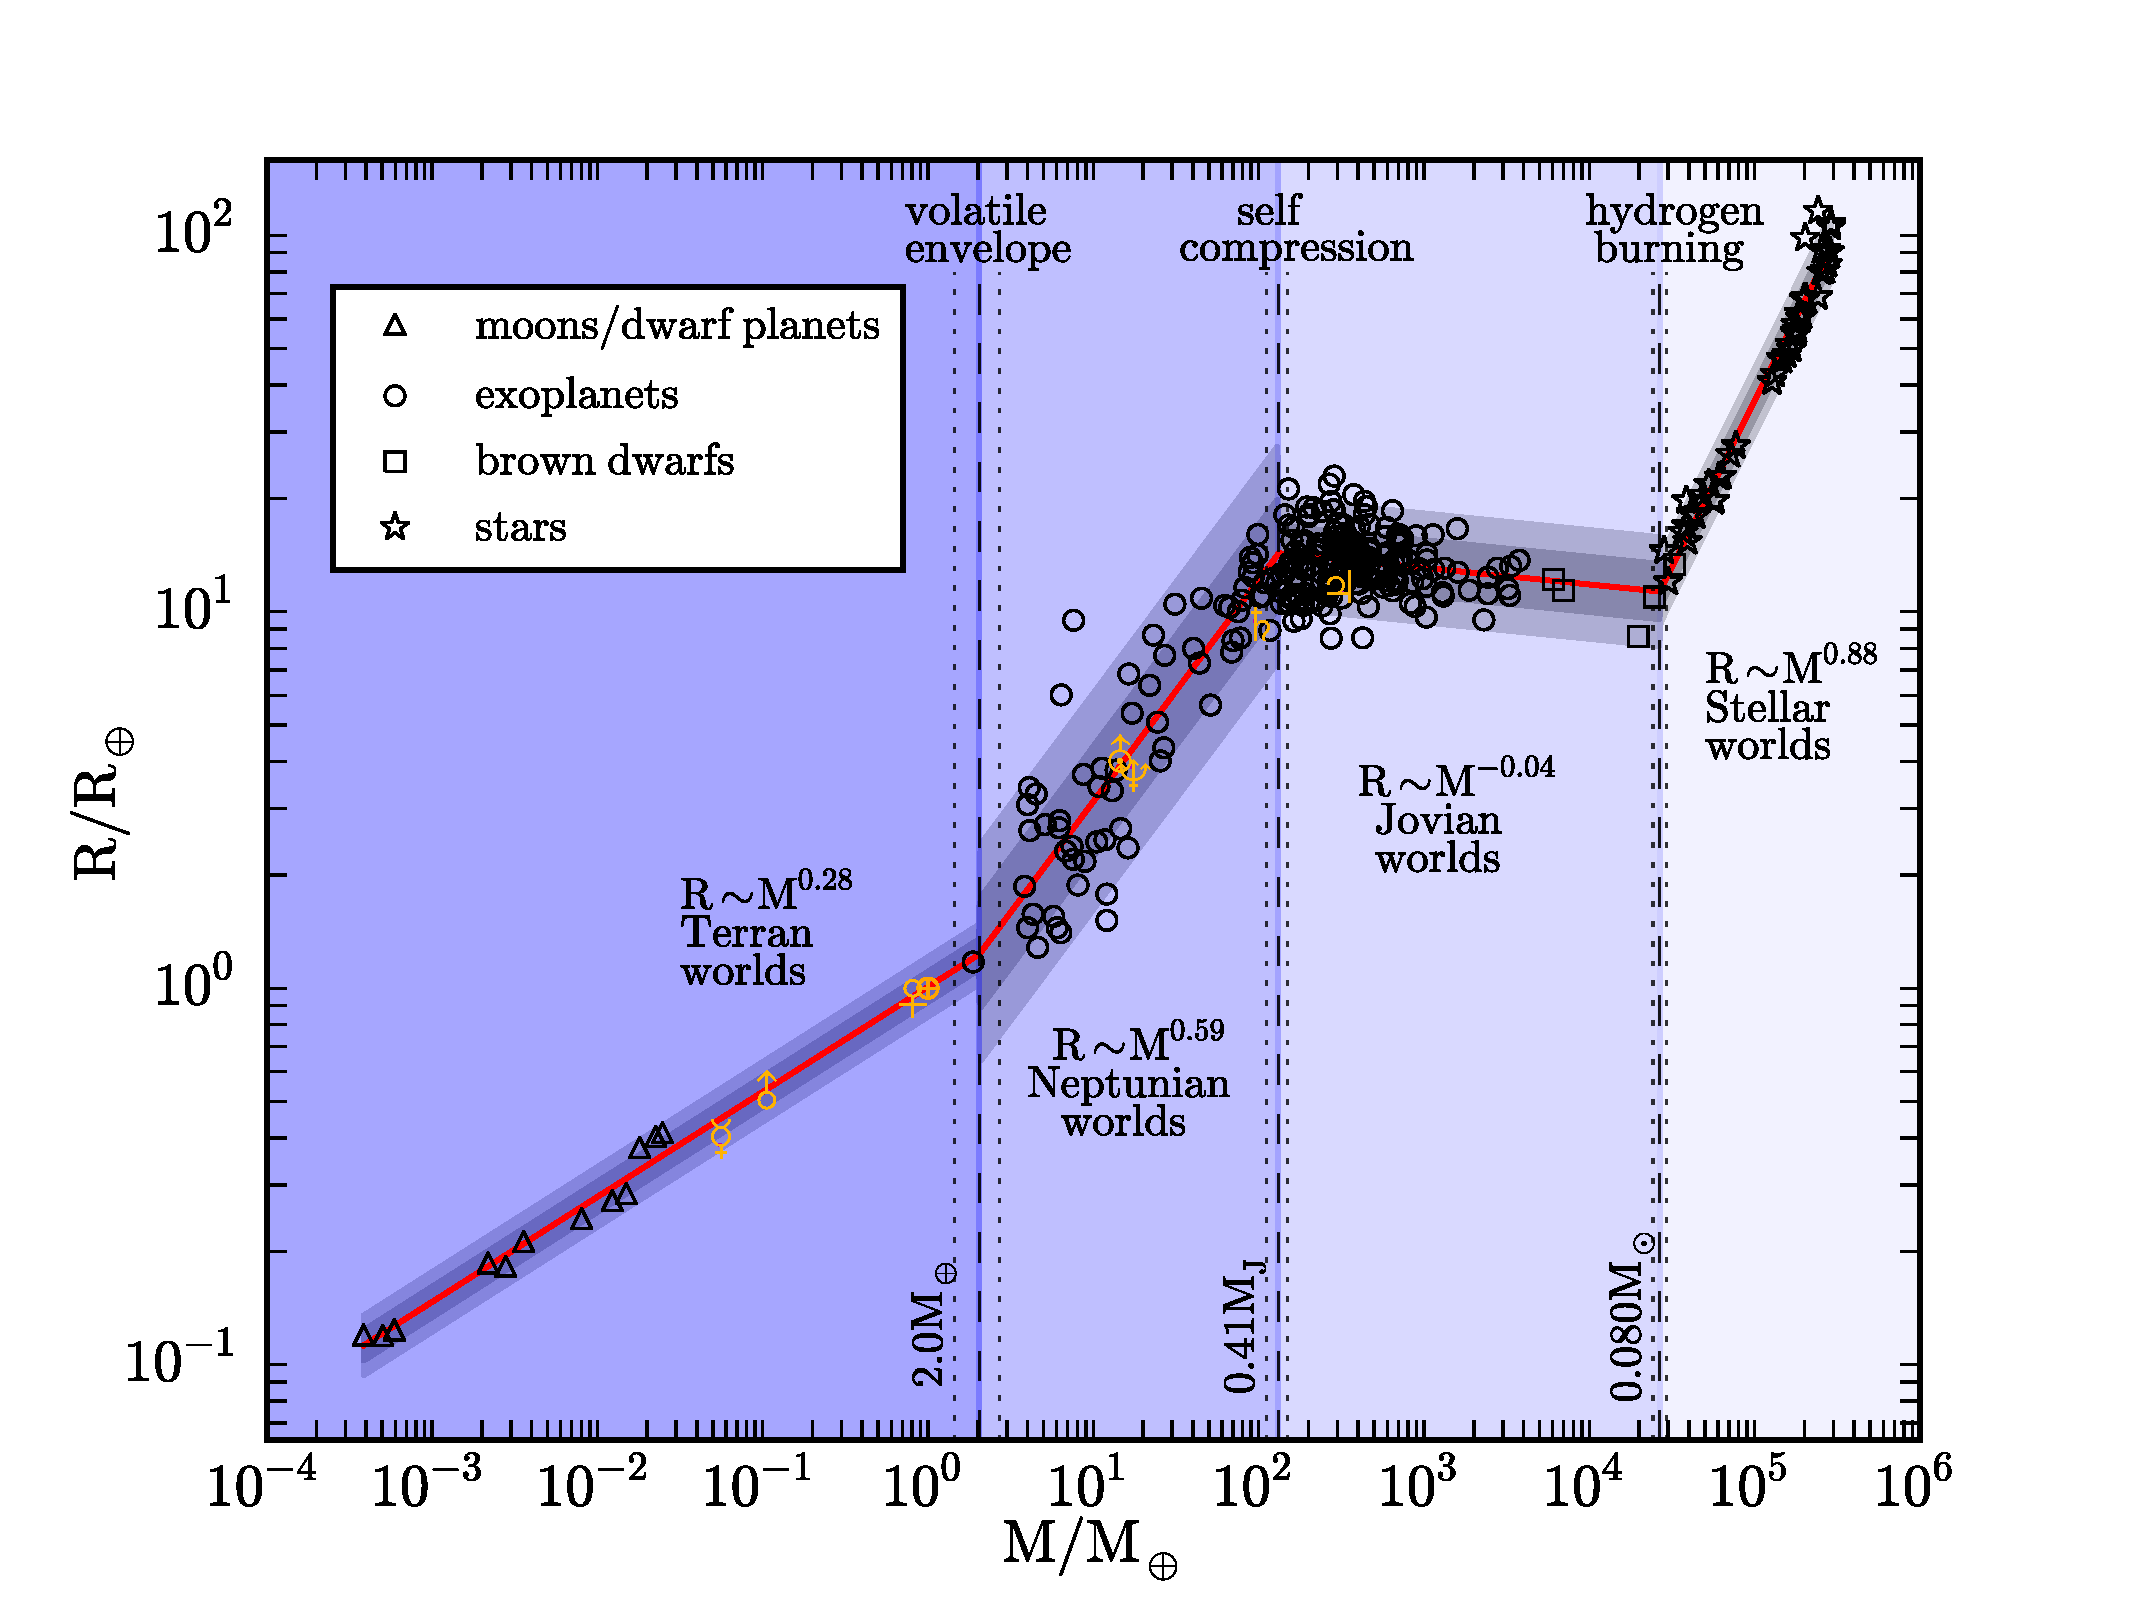
\includegraphics[width=0.9\linewidth]{./figures/introduction/mass_radius_relation.pdf}  \\
    \caption{Left: Mass-Radius relationship from planets to stars~\citet{chen_probabilistic_2016}.}
    \label{fig:mass_radius_relation}
\end{figure}


\citep{santos_observational_2017} Santos et al 2017 \todo{read and quote}  Observational evidence for two distinct giant planet populations
 

double peak histogram from an {RV} paper?? Faria 2018?


did they form from the molecular cloud when the star was forming or from the remnants of the disk after the star formed like exoplanets....?


Theory of migration in the disk through  angular moment transfer (cite).


\section{Conditions for life?}
habitable zone stuff
proxima b
Jorges paragraph....
